% ****** Start of file apssamp-simple.tex ******
%
%   This file is derived from the APS files in the REVTeX 4 distribution.
%   Version 4.0 of REVTeX, August 2001
%
%   It has been simplified for use in Physics 3730/6720 by C. DeTar
%
%   Copyright (c) 2001 The American Physical Society.
%
%   See the REVTeX 4 README file for restrictions and more information.
%
% See the REVTeX 4 README file
%
%  Process this file using 
%
%  1)  pdflatex apssamp-simple.ltx
%
\documentclass[aps,12pt]{revtex4}

\usepackage{graphicx}% Include figure files
\usepackage{bm}% bold math

\begin{document}

\title{Manuscript Title}

\author{N. Author}

\affiliation{Authors' institution and/or address}

\date{\today}

% Note that for RevTeX style the abstract comes before \maketitle.

\begin{abstract}
An article usually includes an abstract, a concise summary of the work
covered at length in the main body of the article. It is used for
secondary publications and for information retrieval purposes. Valid
\end{abstract}

\maketitle

\section{First-level heading}
\label{sec:level1}

This sample document provides an introduction to the use of REV\TeX~4
(and \LaTeXe) in mansucripts prepared for submission to APS
journals.

A random note: A new line is 
invoked with two blackslash characters
\textbackslash\textbackslash
\\ (see \LaTeXe\ source). 

\subsection{Second-level heading}

This is how to make a subsection.

\subsubsection{Third-level heading: References and Footnotes}

To cite bibliography entries, use the \verb+\cite{#1}+ command. The APS
journal styles will display the corresponding number(s) in square
brackets: \cite{ref:feyn54,ref:witten2001}.

Footnotes are produced using the \verb+\footnote{#1}+ command.

\section{Math and Equations}

Inline math may be typeset using the \verb+$+ delimiters. Bold math
symbols may be achieved using the \verb+bm+ package and the
\verb+\bm{#1}+ command it supplies. For instance, a bold $\alpha$ can
be typeset as \verb+$\bm{\alpha}$+ giving $\bm{\alpha}$.

In \LaTeX\ there are many different ways to display equations, and a
few preferred ways are noted below. Displayed math will center by
default. Use the class option \verb+fleqn+ to flush equations left.

Below we have numbered single-line equations; this is the most common
type of equation in \textit{Physical Review}:
\begin{equation}
  Q =  \int\rho\, d^4x = \frac{1}{32 \pi^2}\int F^a_{\mu\nu} \tilde F^a_{\mu\nu} d^4x.
\label{eq:one}.
\end{equation}

When the \verb+\label{#1}+ command is used [cf. input for
Eq.~(\ref{eq:one})], the equation can be referred to in text without
knowing the equation number that \TeX\ will assign to it. Just
use \verb+\ref{#1}+, where \verb+#1+ is the same name that used in
the \verb+\label{#1}+ command.

Unnumbered single-line equations can be typeset
using the \verb+displaymath+ environemnt:
%
\begin{displaymath}
g^+g^+ \rightarrow g^+g^+g^+g^+ \dots ~,~~q^+q^+\rightarrow
q^+g^+g^+ \dots ~.
\end{displaymath}

\subsection{Multiline equations}

Multiline equations are obtained by using the \verb+eqnarray+
environment.  Use the \verb+\nonumber+ command at the end of each line
to avoid assigning a number:
\begin{eqnarray}
E&=&mc, \label{appa}
\\
E&=&mc^2, \label{appb}
\\
E&\agt& mc^3. \label{appc}
\end{eqnarray}

To set a multiline equation without \emph{any} equation
numbers, use the \verb+\begin{eqnarray*}+,
\verb+\end{eqnarray*}+ format:
\begin{eqnarray*}
\sum \vert M^{\text{viol}}_g \vert ^2&=&g^{2n-4}_S(Q^2)~N^{n-2}
        (N^2-1)\\
 & &\times \left( \sum_{i<j}\right)
 \left(
  \sum_{\text{perm}}\frac{1}{S_{12}S_{23}S_{n1}}
 \right)
 \frac{1}{S_{12}}~.
\end{eqnarray*}

The \verb+\label{#1}+ should appear in a section heading, within an
equation, or in a table or figure caption. The \verb+\ref{#1}+ command
is used in the text where the citation is to be displayed.  Some
examples: Section~\ref{sec:level1} on page~\pageref{sec:level1},
Table~\ref{tab:table1}, and Fig.~\ref{fig:arb}.

\section{Figures and Tables}

Figures and tables are typically ``floats'' which means that their
final position is determined by \LaTeX\ while the document is being
typeset. \LaTeX\ isn't always successful in placing floats
optimally.

Figure~\ref{fig:arb} shows a figure. It is embedded using the
\texttt{figure} environment which provides both the caption and the
imports the figure file.

\begin{figure}[h]
\centerline{
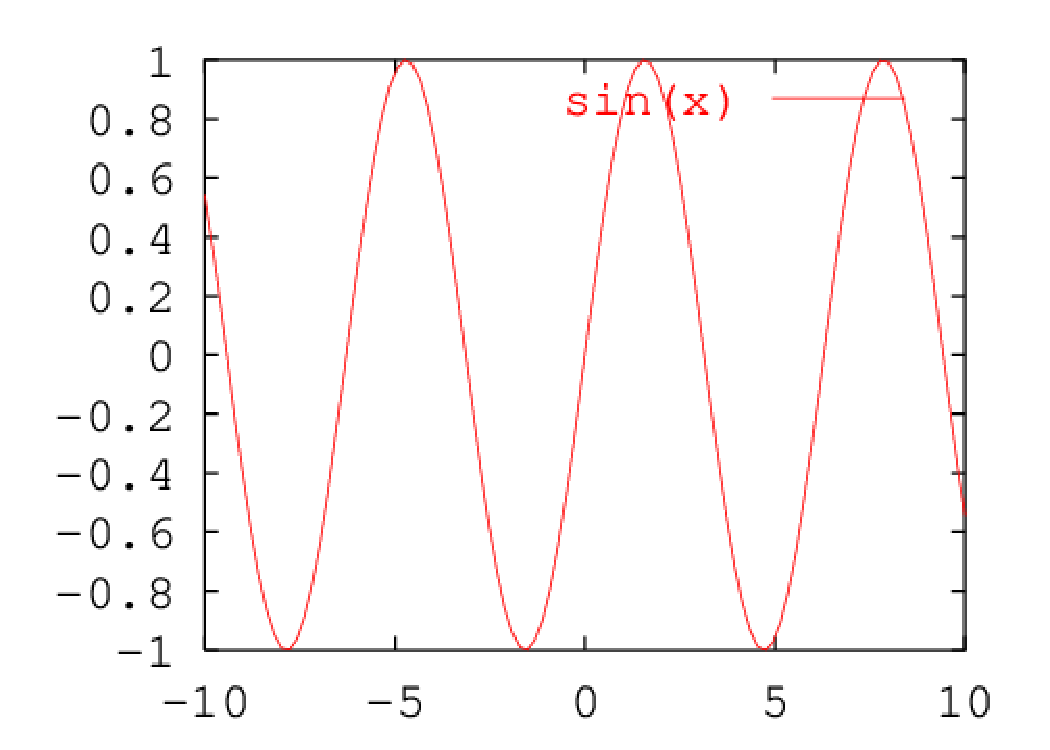
\includegraphics[width=4.5in]{sine.pdf}
% 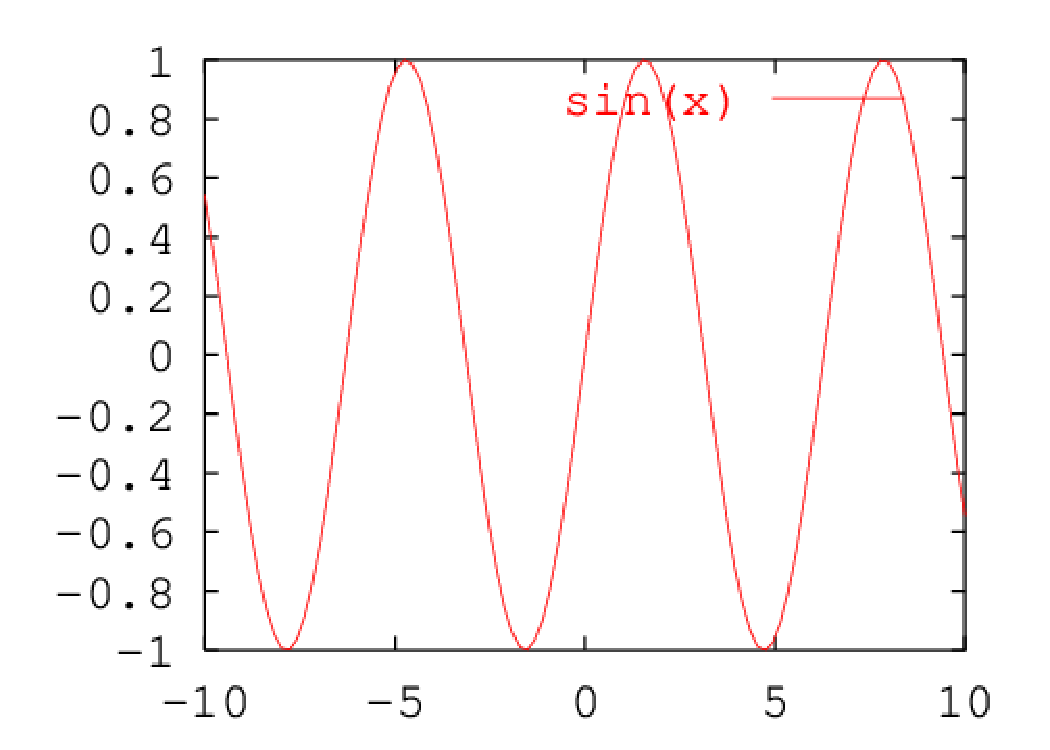
\includegraphics[width=4.5in]{sine.ps}
}
\caption{This is an arbitrary figure.}\label{fig:arb}
\end{figure}

Next we look at tables.  See Table \ref{tab:table1}.

\begin{table}[h]
\caption{\label{tab:table1} This is a table with three columns, the
left one left-justified, the center one centered and the right one
right-justified.}
\begin{ruledtabular}
\begin{tabular}{lcr}
\hline
1 & 2 & 3\\
10 & 20 & 30\\
100 & 200 & 300\\
\end{tabular}
\end{ruledtabular}
\end{table}

\begin{thebibliography}{99}
  \bibitem{ref:feyn54} 
  R.P.~Feynman, Phys.\ Rev. {\bf 94}, 262 (1954).
  \bibitem{ref:witten2001}
  Edward Witten, {\tt hep-th/0106109}.
\end{thebibliography}


\end{document}
%
% ****** End of file apssamp.tex ******
